%%%% Weekly Report Information %%%%
\newcommand{\handoutName}{Weekly report}
\newcommand{\handoutdate}{\today}
%\newcommand{\duedate}{}
% Header template used for Weekly Reports
\documentclass[11pt,twoside]{article}

\setlength{\oddsidemargin}{0pt}
\setlength{\evensidemargin}{0pt}
\setlength{\textwidth}{6.5in}
\setlength{\topmargin}{0in}
\setlength{\textheight}{8.5in}
\setlength{\voffset}{0in}

\providecommand{\titlesize}{small}


\usepackage{graphicx}
%\usepackage{subfigure}
\usepackage{palatino}
%\usepackage{cmbright}
\newcommand{\myMargin}{1.00in}
%\usepackage[pdftex]{hyperref}
\usepackage[small,bf]{caption}
%\usepackage{amsmath}
\usepackage[usenames,dvipsnames]{color}
\usepackage{fancyhdr}
\pagestyle{fancy}
\usepackage{datetime}
\usepackage{fancyvrb}
\usepackage{color}
\usepackage[\titlesize, compact]{titlesec}
\usepackage{multicol}
\usepackage{enumitem}
\usepackage{pdfpages}
\usepackage{mdwlist}
\usepackage{caption}
\usepackage{subcaption}
\usepackage{hyperref}
\usepackage[cmex10]{amsmath}
\usepackage{algorithmicx}
\usepackage[ruled]{algorithm}
\usepackage{algpseudocode}
\renewcommand\labelenumi{\textbf{\theenumi) }}
\newcommand\algorithmicinput{\textbf{Input:}}
%\newcommand\INPUT{\item[\algorithmicinput]}
\newcommand\algorithmicassume{\textbf{Assume:}}
%\newcommand\ASSUME{\item[\algorithmicassume]}

\newdateformat{dashdate}{\THEYEAR-\twodigit{\THEMONTH}-\twodigit{\THEDAY}}
\def\Tiny{\fontsize{3pt}{3pt}\selectfont}

\providecommand{\handoutName}{Handout title}
\providecommand{\handoutdate}{Handout date}
\providecommand{\duedate}{}

\lhead{Meeting with Prof. Becker\\
Spring, 2017}
\chead{}
\rhead{ Shiva Shahrokhi\\
\handoutdate }
\lfoot{}
\cfoot{\thepage}
\rfoot{\dashdate \Tiny \textcolor{Gray}{\today}}
\renewcommand{\headrulewidth}{0.4pt}
\renewcommand{\footrulewidth}{0.4pt}

\begin{document}

\vspace{0.60in}
\begin{center}
{\Large\textbf{\handoutName}}\\
\vspace{0.03in}
\textbf{\duedate}\\
\end{center}

\newcommand{\todo}[1]{
  \textcolor{Red}{
    \begin{tabular}{|c|}
      \hline
      \em \large \bfseries todo: \normalfont \normalsize #1 \\
      \hline
    \end{tabular}}
}


\section{My \emph{Objectives} this week: Optimal Solution for the algorithm for two robots positioning using friction}
\begin{itemize}
\item Compute reachable regions for the optimal solution.
\item Write down the code of optimal solution.
\end{itemize}



\section{My \emph{Accomplishments} this week}


\begin{itemize}
\item learnt more about mathematica, coding and understanding.
\item the code for reachable regions for all 4 walls.
\end{itemize}
The reachable regions with regard to $\Delta x ,\Delta y$ is shown here. \\
For horizontal (top and bottom) walls: $\Delta x \in [r2_x - r1_x -1 , 1]$ and $\Delta y \in [r2_y - r1_y , 0]$.\\
For vertical (right and left) walls: $\Delta x \in [0 , r2_x - r1_x]$ and $\Delta y \in [-1 , r2_y - r1_y +1]$.\\
This figure shows the snapshot of the reachable sets:
\begin{figure}[h]
\begin{center}
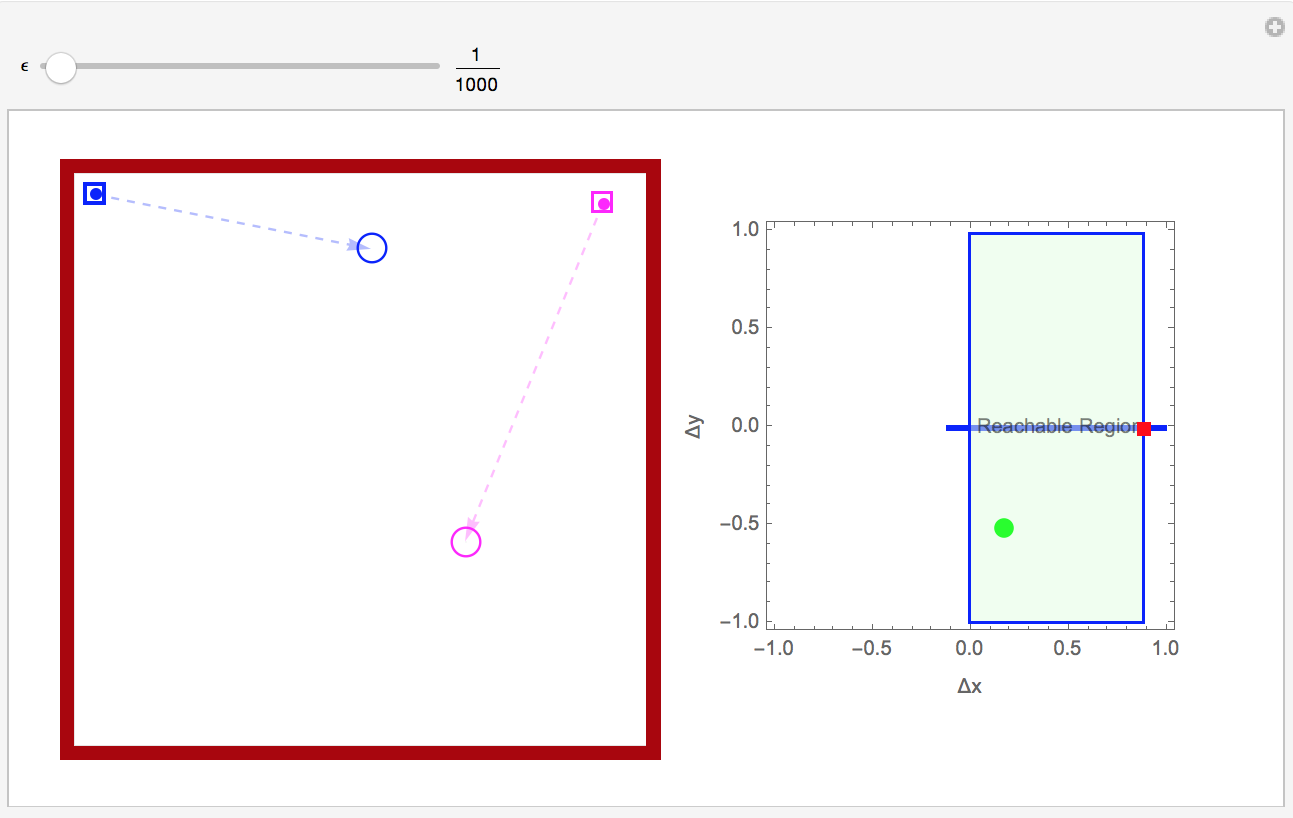
\includegraphics[width=10cm]{ReachableSet.png}
\caption{The two rectangles shows the reachable sets of the robots.}
\end{center}
\end{figure}


\section{My \emph{Plan} for next week}

\begin{itemize}
\item complete the dynamic programming part of the new solution. Is this possible to get to the goal with 5 moves? Can we get near to the optimal solution by our current idea? 
\item write down the new algorithm if it worked and was optimal, and make the first draft for IROS.
\item have fun with kilobots for the outreach on Saturday!
\end{itemize}

\subsection{Meeting with Dr. Becker  }

\begin{itemize}
\item Get help on the implementation of the algorithm to make sure it is ok. 
\end{itemize}

\end{document}
